\documentclass[10pt]{article}

\usepackage[margin=0.82in]{geometry}
\usepackage[T1]{fontenc}
\usepackage[utf8]{inputenc}
\usepackage{amsmath,amssymb,amsthm,booktabs,graphicx}
\usepackage{float}
\usepackage{algorithm}
\usepackage{algpseudocode}
\usepackage[section]{placeins}
\usepackage[hidelinks]{hyperref}
\usepackage{microtype}

\newtheorem{theorem}{Theorem}

\title{Adaptive Best-of-$N$ with Unknown Reward\\
and Unknown Generation-Cost Distributions}
\author{}
\date{}

\begin{document}
\maketitle

\begin{abstract}
We study adaptive generation when neither the prompt-specific reward
distribution nor the cost of the next response is known.  Opening a box
reveals a reward and a response length, and the objective is the best revealed
reward minus the total realized generation cost.  We first formulate the
i.i.d. Pandora problem with random opening costs.  Its known-distribution rule
uses the mean random cost in the usual fair-cap equation.  We then state the
learned-threshold guarantee of \emph{Learning When to Stop} for this setting;
the proof is unchanged after the constant cost is replaced by the mean random
cost and the fair-cap estimator is allowed to use both rewards and costs.

For language-model tasks, the main practical difficulty is putting reward and
cost into comparable units.  We give a detailed account of that calibration.
Alignment uses a Bradley--Terry probability against a prompt-specific
high-quality benchmark, while coding uses a train-only isotonic estimate of
the probability of correctness.  The simplified alignment rule fits its
upper tail entirely from the current prompt and needs no training stage.  The
coding rule learns one global upper tail after isotonic calibration; the same
configuration is used at every character cost.  Both estimate the next
response length by its running mean and generate once more only when estimated
gain exceeds estimated character cost.  We give one common blueprint and
exact descriptions of these two rules.

The experiments compare adaptive stopping with deployable and oracle fixed
policies.  Alignment uses a train-selected Fixed-$N$, a test-oracle Fixed-$N$,
and a stronger test-oracle character-budget allocation that knows each
prompt's mean response length.  Coding uses train-selected and test-oracle
Fixed-$N$ baselines and a fixed character budget selected on the training
half and transferred unchanged to test.  The Alignment section reports
utility, head-to-head win rate at exactly matched expected character cost,
and target quality; the Coding section reports utility and target accuracy.
In both target experiments, the Fixed-$N$ comparator is selected on the
training half and frozen for test.  Target calibration plots are shown beside
character savings so that train-to-test overshoot or undershoot is visible.
We additionally give post-hoc Fixed-$N$ diagnostics at exactly the adaptive
test quality, separating allocation efficiency from calibration error.  All
reported costs are exact cumulative output characters, including for policies
whose stopping decisions use estimated costs.
\end{abstract}

\section{Pandora's box with unknown rewards and unknown costs}
\label{sec:model}

We begin with the clean stopping problem.  A single type of box is available
repeatedly.  Opening box $i$ reveals a reward $X_i$ and incurs a nonnegative
cost $C_i$.  The pairs
\begin{equation}
  (X_1,C_1),(X_2,C_2),\ldots
  \quad\text{are independent and identically distributed,}
  \label{eq:iid-pairs}
\end{equation}
but their joint distribution is unknown.  Reward and cost may be dependent
within a pair.  Before opening box $i$, neither $X_i$ nor $C_i$ is known.  Once
the box is opened, both are observed and its cost is paid.  The decision after
each opening is whether to stop or to open one more box.

Let
\begin{equation}
  M_n=\max_{1\le i\le n}X_i
\end{equation}
be the best observed reward.  A stopping time $T\ge1$ receives payoff
\begin{equation}
  R_T=M_T-\sum_{i=1}^{T}C_i.
  \label{eq:random-cost-objective}
\end{equation}
We assume $\mathbb E[X^+]<\infty$ and
$\bar c=\mathbb E[C]\in(0,\infty)$.  Define
\begin{equation}
  L(s)=\mathbb E[(X-s)_+],
  \qquad S(s)=\Pr(X\ge s),
  \qquad
  \tau=\sup\{s:L(s)\ge\bar c\}.
  \label{eq:random-cost-cap}
\end{equation}
The function $L$ measures the value of one more reward draw above a current
best value $s$.  We call $\tau$ the fair cap.  For the continuous
distributions considered here, $L(\tau)=\bar c$.

If the joint distribution were known, the optimal rule would stop at
\begin{equation}
  T_W=\inf\{n\ge1:M_n\ge\tau\}.
  \label{eq:oracle-stop}
\end{equation}
This is the usual i.i.d. Pandora rule with the deterministic cost replaced by
the mean random cost.  To see why this replacement is sufficient, condition
on the observations before the next opening.  The expected change from one
more box at incumbent $m$ is
\begin{equation}
  \mathbb E[(X-m)_+-C]=L(m)-\bar c.
  \label{eq:one-step-random-cost}
\end{equation}
No independence between $X$ and $C$ inside a box is needed for this identity.
The stopping decision is made before either member of the next pair is
observed, and the cost enters additively.  Under the standard integrability
conditions, the known-distribution expected payoff is
$\mathbb E[R_{T_W}]=\tau$.

\subsection{The learned-threshold theorem}

The main theorem of \emph{Learning When to Stop} extends directly to the
model above.  The only statistical change is that the fair-cap estimate must
now learn both the reward distribution entering $L$ and the mean cost
$\bar c$.  We state the result and do not repeat its proof.

After $n$ observed reward--cost pairs, let $\widehat\tau_n$ be any estimate of
the solution to $L(t)=\bar c$.  For a nonnegative bonus $b_n$, define
\begin{equation}
  U_n=\widehat\tau_n+b_n,
  \qquad
  T=\inf\{n\ge1:M_n\ge U_n\}.
  \label{eq:learned-threshold-rule}
\end{equation}
For deterministic widths $w_1,w_2,\ldots$, define the local band cost
\begin{equation}
  \Gamma_{\mathcal D}(w)
  =S(\tau)\sum_{n\ge1}
    w_n\Pr\{\tau\le M_n<\tau+w_n\}.
  \label{eq:local-band}
\end{equation}
It charges an upward threshold error only on histories where that error
actually makes the learned rule continue after the oracle would stop.

\begin{theorem}[Unknown-reward and unknown-cost reduction]
\label{thm:random-cost-reduction}
Suppose there is a scale $a>0$ such that, for every $n\ge1$ and $x\ge0$,
\begin{equation}
 \Pr\!\left(
  |\widehat\tau_n-\tau|>
  a\left\{\sqrt{\frac{2x}{n}}+\frac{2x}{n}\right\}
 \right)\le2e^{-x}.
 \label{eq:random-cost-concentration}
\end{equation}
Use
\begin{equation}
 b_n=a\left\{
       4\sqrt{\frac{\log(en)}{n}}
       +\frac{16\log(en)}{n}
     \right\},
 \qquad U_n=\widehat\tau_n+b_n,
 \qquad w_n=2b_n.
 \label{eq:random-cost-bonus}
\end{equation}
If $\Pr(X>\tau)>0$, the stopping rule in
Eq.~\eqref{eq:learned-threshold-rule} stops almost surely and
\begin{equation}
  \mathbb E[R_{T_W}-R_T]
  \le \Gamma_{\mathcal D}(w)+a.
  \label{eq:random-cost-guarantee}
\end{equation}
Consequently, whenever the right-hand side is at most $\varepsilon\tau$, the
learned rule obtains at least a $(1-\varepsilon)$ fraction of the oracle
payoff.
\end{theorem}

The theorem is deliberately a reduction.  It does not say that every unknown
reward and cost distribution is easy.  It says that once a structured model
gives a concentrated estimate of the fair cap, including the uncertainty in
mean cost, the stopping loss is controlled by the estimation scale and by a
local decision term.  The practical LLM algorithms below use this same
crossing principle, but use regularized fitted tails rather than claiming the
finite-sample confidence statement in
Eq.~\eqref{eq:random-cost-concentration}.


\section{Putting LLM reward and generation cost on one scale}
\label{sec:calibration}

In a language-model application, opening a box means generating and scoring
one response.  Its length is not known until generation finishes.  Let $K_i$
be the output character count of response $i$.  For a supplied divisor $D$,
we convert it to utility cost
\begin{equation}
  C_i=\frac{K_i}{D}.
  \label{eq:character-cost}
\end{equation}
Thus $D$ is the number of characters worth one unit of utility.  It is an
external economic scale, not a prediction of response length.  The random
variable $K_i$ is the unknown opening cost.  During evaluation we always
charge the exact sum $\sum_{i\le T}K_i/D$; an estimated length is used only to
decide whether to generate the next response.

The other side of the comparison is harder.  A raw reward-model score has no
natural unit relative to characters.  It can be negative, its scale changes
across reward models, and a one-point increase need not have the same meaning
on different prompts.  We therefore map the raw score to a bounded,
task-relevant utility before comparing the value of another response with
$K_i/D$.  Alignment and coding require different maps because their outcomes
have different meanings.

\subsection{Alignment: Bradley--Terry utility}
\label{sec:bt-calibration}

Let $Y$ be a raw alignment reward and let $\beta$ be the score of a
high-quality response for the same prompt.  We use
\begin{equation}
  u_\beta(y)=\sigma(y-\beta)
  =\frac{1}{1+\exp(\beta-y)}.
  \label{eq:bt-map}
\end{equation}
This is the unit-temperature Bradley--Terry probability that a response with
score $y$ beats a response with score $\beta$.  There are three reasons for
this choice.

First, alignment reward models are designed to rank responses according to
preference.  A pairwise win probability is therefore closer to their intended
semantics than treating the raw score itself as cardinal utility.  Second,
the difference $y-\beta$ removes prompt-specific score offsets.  A score of
five is not intrinsically good, but being well above a high benchmark for the
same prompt is meaningful.  Third, the sigmoid bounds utility in $(0,1)$,
which gives a stable and interpretable scale for comparison with character
cost.

The benchmark is the prompt's 99th reward percentile.  It is deliberately
difficult: $u_\beta(y)=1/2$ means that the candidate is estimated to tie a
response near the top one percent of that prompt's reward distribution.  The
online algorithm does not know this percentile.  It estimates it from the
observed score prefix using a regularized upper-tail model.  A full-pool 99th
percentile is used only after stopping to evaluate all policies on a common
scale.  We use a unit-temperature link and do not fit a Bradley--Terry
temperature; consequently, the map is best understood as a transparent
BT-style utility scale rather than a separately validated probability model.

\subsection{Coding: probability of correctness from isotonic regression}
\label{sec:isotonic-calibration}

For coding, the final reward is binary correctness.  The natural utility of a
candidate with raw score $y$ is therefore its probability of being correct.
On each outer split, we use all labeled generations from the 41 training
problems to fit
\begin{equation}
 \widehat g\in
 \arg\min_{\substack{g:\mathbb R\to[0,1]\\g\ \mathrm{nondecreasing}}}
 \sum_{i\in\mathcal A}\sum_{j=1}^{512}
 \{Z_{ij}-g(Y_{ij})\}^2,
 \qquad Z_{ij}\in\{0,1\}.
 \label{eq:isotonic-map}
\end{equation}
The calibrated utility is $P_{ij}=\widehat g(Y_{ij})$.

Isotonic regression is appropriate here because the reward score is intended
to rank candidate programs, but there is no reason to assume that equal score
increments correspond to equal changes in correctness probability.  The
monotonicity constraint preserves the reward model's ordering, while the
piecewise-constant fit learns the shape of the score--correctness relationship
without imposing a sigmoid or choosing reward bins.  It also maps directly to
the quantity used by the coding objective:
\begin{equation}
  \mathbb E[Z\mid Y=y]\approx\widehat g(y).
\end{equation}
Unlike alignment, coding has observed binary training labels, so a direct
probability calibration is preferable to a relative BT comparison.

The isotonic map is fit only on the training half, then frozen.  Scores outside
the training range receive the corresponding endpoint prediction.  The test
policy observes a program's raw reward and length, applies the frozen map, and
never observes correctness.  Correctness is revealed only to the offline
evaluator.  Isotonic plateaus can tie several programs; the implementation
returns the first opened program attaining the largest calibrated value.

\subsection{A common algorithmic blueprint}
\label{sec:blueprint}

After calibration, the two applications have the same structure.  The policy
opens a short prefix and forms an optimistic fitted distribution for the
utility of the next response.  Alignment forms this distribution from the
current prefix alone; coding uses one tail learned on training problems.  If
$c_n$ is the estimated utility cost of one more response, the fitted
reservation value, or fair cap, is
\begin{equation}
 \tau_n=\inf\left\{t:
   \mathbb E_{\widehat F_n}[(U-t)_+] + \varepsilon_n\le c_n
 \right\},
 \label{eq:fitted-fair-cap}
\end{equation}
where $\varepsilon_n$ is the policy's small optimism correction.  The policy
stops exactly when its best observed utility is at least $\tau_n$.  Thus the
fair cap combines the predicted benefit and cost of one more generation into
one interpretable threshold.

\begin{algorithm}[t]
\caption{Blueprint for adaptive LLM generation}
\label{alg:llm-blueprint}
\begin{algorithmic}[1]
\Require Any task-specific training data; character divisor $D$; horizon $H$;
initial count $m_0$
\State Fit the task-specific calibration and tail information, if required
\State Generate $m_0$ responses and observe their scores and character counts
\State Map each observed score to the task's bounded utility scale
\For{$n=m_0,m_0+1,\ldots,H-1$}
  \State Fit the task's optimistic utility distribution $\widehat F_n$
  \State Let $v_n$ be the largest calibrated utility among the first $n$
         responses
  \State Set $c_n$ to the observed mean response length divided by $D$
  \State Find the fair cap $\tau_n$ from
         $\mathbb E_{\widehat F_n}[(U-\tau_n)_+]+\varepsilon_n=c_n$
         \Comment{use the boundary convention in \eqref{eq:fitted-fair-cap}}
  \If{$v_n\ge \tau_n$}
    \State Stop and return the best response observed so far
  \EndIf
  \State Generate response $n+1$ and observe its score and exact length
\EndFor
\State Return the best observed response and charge the exact total character
       count
\end{algorithmic}
\end{algorithm}

Algorithm~\ref{alg:llm-blueprint} is a single adaptive stopping rule, not a
mixture with Fixed-$N$.  Fixed-$N$ appears only as an evaluation baseline.
The two concrete policies differ in the calibration map, the fitted upper
tail, and a small number of regularization choices described next.


\section{Alignment}
\label{sec:alignment}

\subsection{Exact alignment policy}
\label{sec:alignment-algorithm}

Algorithm~\ref{alg:alignment} states the decision at the distribution level.
The rule has no training stage.  At each prefix it fits a shifted exponential
to the inclusive upper half of the current prompt's exponentiated scores,
uses the fitted law to obtain a fair cap, and compares the incumbent with that
cap.  The confidence multiplier $\gamma$ is an explicit input; all experiments
use its default value $0.6$.

\begin{algorithm}[H]
\caption{Alignment: training-free adaptive stopping rule}
\label{alg:alignment}
\footnotesize
\begin{algorithmic}[1]
\Require Divisor $D$; horizon $H=960$; initial count $m_0=5$;
confidence $\gamma$ (default $0.6$)
\State Generate $m_0$ responses and observe scores and lengths $(Y_j,K_j)$
\State $n\gets m_0$
\While{$n<H$}
  \State $E_j\gets\exp\{\operatorname{clip}(Y_j,-50,50)\}$ for $j\le n$
  \State $T_n\gets$ the $\lfloor n/2\rfloor+1$ largest observed $E_j$
         \Comment{inclusive upper half}
  \State $\ell_n\gets\min T_n$ \Comment{fitted shift}
  \State $\widehat\lambda_n\gets
         \max\{\operatorname{mean}(T_n)-\ell_n,10^{-8}\}^{-1}$
         \Comment{fitted rate}
  \State $\widehat X_n\sim
         \operatorname{ShiftedExp}(\ell_n,\widehat\lambda_n)$
  \State $h_n\gets\sqrt{\log(20)/|T_n|}$
  \State $s_n^+\gets\widehat\lambda_n^{-1}(1+\gamma h_n)$
         \Comment{optimistic tail scale}
  \State $s_n^-\gets
         \max\{\widehat\lambda_n^{-1}(1-\gamma h_n),10^{-8}\}$
         \Comment{conservative benchmark scale}
  \State $b_{n,\gamma}\gets\log(\ell_n+s_n^-\log 50)$
  \State Define $\widehat F_{n,\gamma}$ by: with probability $1/2$, $U=0$;
         otherwise draw $Z\sim\operatorname{Exp}(1)$ and set
         $U=\sigma\{\log(\ell_n+s_n^+Z)-b_{n,\gamma}\}$
  \State $c_n\gets (nD)^{-1}\sum_{j=1}^{n}K_j$
         \Comment{estimated cost of one more response}
  \State $\varepsilon_n\gets0.002\sqrt{\log(20)/(2n)}$
  \State $\displaystyle \tau_n\gets\inf\left\{t\in[0,1]:
         \mathbb E_{U\sim\widehat F_{n,\gamma}}[(U-t)_+]
         +\varepsilon_n\le c_n\right\}$
         \Comment{fair cap of $\widehat F_{n,\gamma}$ at cost $c_n$}
  \State $v_n\gets\sigma(\max_{j\le n}Y_j-b_{n,\gamma})$
  \If{$v_n\ge\tau_n$}
    \State \textbf{break} \Comment{incumbent has reached the fair cap}
  \EndIf
  \State Generate response $n+1$ and observe $(Y_{n+1},K_{n+1})$
  \State $n\gets n+1$
\EndWhile
\State $J\gets\min\arg\max_{j\le n}Y_j$
\State Return response $J$ and charge exact cost $\sum_{j=1}^{n}K_j/D$
\end{algorithmic}
\end{algorithm}

The upper-tail component of $\widehat F_{n,\gamma}$ has probability $0.5$;
the remaining probability is placed at zero and contributes nothing to the
positive part.  The factor $\log 50$ extrapolates from tail mass $0.5$ to the
implied 99th percentile.

Because the expected positive part decreases with $t$, the test
$v_n\ge\tau_n$ is algebraically identical to evaluating it once at $v_n$ and
comparing the result with $c_n$.  The implementation therefore does not need
a numerical root finder; $\tau_n$ is the cleaner conceptual statement of the
same stopping decision.

Five initial responses, default confidence $\gamma=0.6$, and bonus $0.002$ are
frozen for every generator, divisor, and final split.
There is no reward prior, cost prior, fitted temperature, or other training
quantity in the stopping decision.  This is one UCB-style Pandora crossing
rule: it does not consult Fixed-$N$, impose a Fixed-$N$ guard, or inspect the
next response length before opening it.

\subsection{Utility experiment and fixed-policy baselines}
\label{sec:alignment-experiment}

We evaluate 100 Alpaca prompts for each of five generators: Gemma-2-9B,
Llama-3.1-8B, Llama-3.2-3B, Mistral-7B, and Qwen-2.5-7B.  Every prompt has
960 responses scored by RM-Mistral-7B.  Ten deterministic splits divide the
prompts into 50 training and 50 test prompts.  The training half selects the
implementable Fixed-$N$ baseline and, in the target experiment, the adaptive
divisor.  It fits nothing used by Algorithm~\ref{alg:alignment}, whose formula
is fixed across generators, divisors, and final splits.  We replay four
permutations per training prompt and eight per test prompt.  The evaluated
divisors are
\begin{equation}
 D\in\{10^5,5\!\times\!10^5,10^6,5\!\times\!10^6,10^7,5\!\times\!10^7\}.
\end{equation}

For evaluation only, prompt $x$ has full-pool benchmark $\beta_x^\star$, the
fixed empirical 99th percentile of its 960 rewards.  If a policy returns raw
reward $y$, its evaluated utility is
\begin{equation}
 U_x(y,T)=\sigma(y-\beta_x^\star)
          -\frac{1}{D}\sum_{j=1}^{T}K_j.
 \label{eq:alignment-evaluation}
\end{equation}
The online policy never sees $\beta_x^\star$.  It uses $b_n$ from
Algorithm~\ref{alg:alignment}.

We compare the adaptive rule with three fixed policy classes.

\paragraph{1. Train-selected Fixed-$N$ (implementable).}
For every split and divisor, choose the integer $N\in\{1,\ldots,960\}$ that
maximizes mean utility on the 50 training prompts.  Freeze that $N$ and run it
on the test prompts.  This rule uses no test outcome to choose $N$.

\paragraph{2. Test-oracle Fixed-$N$.}
Choose the single integer $N$ that maximizes mean utility on the test prompts
and the same held-out permutations used for evaluation.  This is not
implementable; it measures the best uniform generation count available after
seeing the test results.

\paragraph{3. Test-oracle fixed character budget.}
This stronger oracle knows each test prompt's mean full-pool response length
\begin{equation}
  \ell_x=\frac1{960}\sum_{j=1}^{960}K_{xj}.
\end{equation}
Given one common character budget $R$, it allocates
\begin{equation}
 N_x(R)=\max\left\{1,
        \min\left\{960,\left\lfloor\frac{R}{\ell_x}\right\rfloor\right\}
        \right\}
 \label{eq:oracle-budget-allocation}
\end{equation}
generations to prompt $x$.  The test set itself chooses $R$ to maximize mean
utility.  We enumerate the exact allocation breakpoints
$R=n\ell_x$, rather than using an approximate grid.  Although $R$ determines
the allocation, evaluation charges the actual cumulative character counts,
not $R$.  This baseline is oracle in two ways: it knows each test prompt's
mean length and tunes the common budget on test outcomes.

For baseline $B$, we first compute the percentage relative improvement within
each prompt split $s$,
\begin{equation}
  I_{s,B}=100\,
  \frac{\overline U_{{\rm adaptive},s}-\overline U_{B,s}}
       {\overline U_{B,s}},
  \label{eq:relative-improvement}
\end{equation}
and report its mean across splits.  This is easier to read than a ratio: zero
denotes equality and positive values favor adaptive stopping on this
split-normalized metric.  Figure~\ref{fig:alignment-baselines} shows pointwise
95\% Student-$t$ intervals across the ten prompt splits.

\begin{figure}[H]
 \centering
 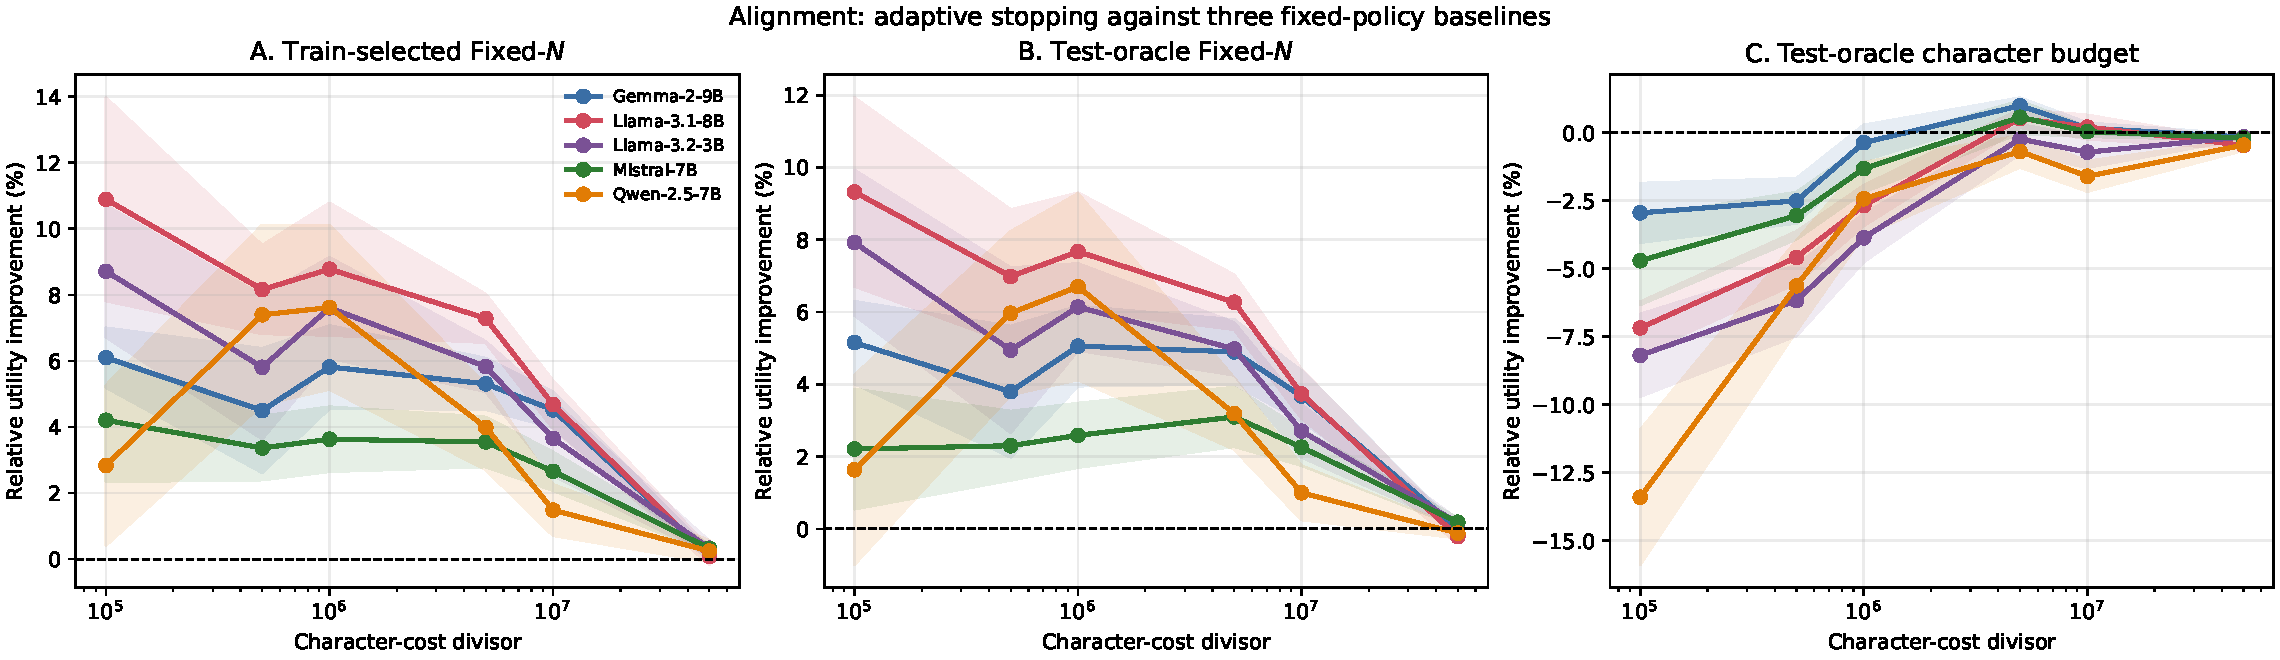
\includegraphics[width=\textwidth]
   {figures/alignment/alignment_revised_baselines.pdf}
 \caption{Alignment percentage relative utility improvement over the three
 requested baselines.  The first baseline selects $N$ on the training half;
 the other two select their parameter on the test half and are intentionally
 optimistic.  The dashed zero line denotes equal utility.}
 \label{fig:alignment-baselines}
\end{figure}

Table~\ref{tab:alignment-summary} averages the six displayed divisor-level
percentage improvements for each generator.  The training-free rule exceeds
train-selected Fixed-$N$ in all 30 generator--divisor cells and the
test-oracle Fixed-$N$ in 28 of 30.  Averaged equally across the 30 cells, the
improvements are 4.65\% and 3.81\%, respectively.  The prompt-specific
character-budget oracle is stronger: adaptive utility is 2.37\% lower on
average and exceeds it in 6 of 30 cells.  Relative to the previous
training-shrunk rule, the mean utility change is only $-0.00040$ in absolute
units, while the entire alignment training stage disappears.

\begin{table}[H]
\centering
\small
\begin{tabular}{lccc}
\toprule
Generator & Train-selected $N$ & Oracle $N$ & Oracle character budget\\
\midrule
Gemma-2-9B   & $+4.39\%$ & $+3.76\%$ & $-0.80\%$\\
Llama-3.1-8B & $+6.65\%$ & $+5.63\%$ & $-2.36\%$\\
Llama-3.2-3B & $+5.32\%$ & $+4.48\%$ & $-3.22\%$\\
Mistral-7B   & $+2.95\%$ & $+2.11\%$ & $-1.45\%$\\
Qwen-2.5-7B  & $+3.93\%$ & $+3.06\%$ & $-4.03\%$\\
\midrule
All generator--divisor cells & $+4.65\%$ & $+3.81\%$ & $-2.37\%$\\
\bottomrule
\end{tabular}
\caption{Alignment percentage relative utility improvement, averaged equally
over the six displayed character divisors.}
\label{tab:alignment-summary}
\end{table}

\subsection{Win rate at matched expected characters}
\label{sec:alignment-win-rate}

Utility combines quality and cost, so a utility gain alone does not reveal
whether adaptive stopping returns better responses, spends fewer characters,
or both.  For each generator, split, and divisor, we therefore replay
Fixed-$N$ independently.  On the test set, a randomized mixture of the two
adjacent integer values of $N$ is chosen so that its expected character count
equals the adaptive policy's test character count exactly.  We then compare
the two returned raw rewards head to head, with a tie contributing one half.
Because the mixing weight uses test cost after the fact, this is an oracle
diagnostic rather than a deployable baseline.

\begin{figure}[H]
 \centering
 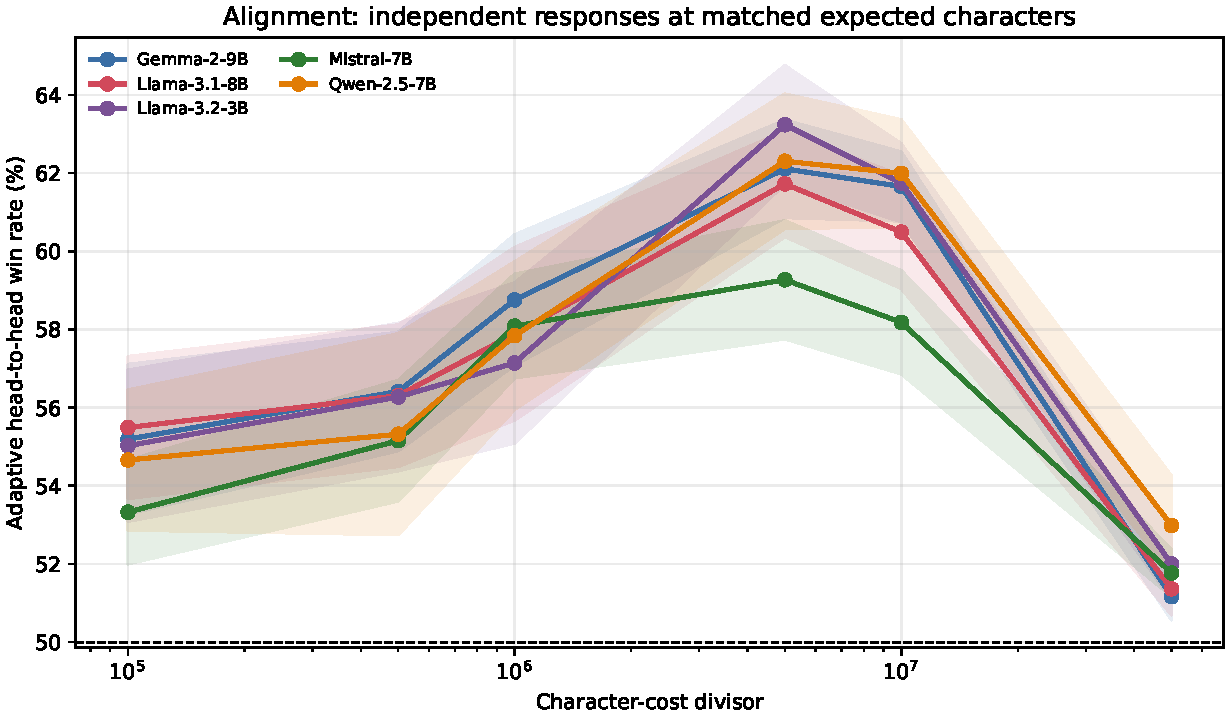
\includegraphics[width=0.82\textwidth]
   {figures/alignment/alignment_equal_cost_win_rate.pdf}
 \caption{Alignment head-to-head win rate against independent Fixed-$N$
 responses at exactly matched expected characters.  Bands are pointwise 95\%
 Student-$t$ intervals over ten splits; 50\% denotes equality.}
 \label{fig:alignment-win-rate}
\end{figure}

Across the 30 generator--divisor cells, mean adaptive win rates range from
51.16\% to 63.24\%.  The lower endpoint of every displayed 95\% interval is
above 50\%.  Thus the utility improvement over uniform Fixed-$N$ is not only
an artifact of spending fewer characters: with expected cost held fixed,
adaptive allocation selects the better response more often.

\subsection{Target quality and character saving}
\label{sec:alignment-target}

Here target quality means the test average of the BT evaluation utility in
Eq.~\eqref{eq:alignment-evaluation} before subtracting cost.  For each outer
training half, generator, and target in
$\{0.30,0.35,\ldots,0.60\}$, we make two independent selections.  Among the
eleven adaptive divisors from $5\times10^4$ through $5\times10^7$, we select
the single policy with the lowest training mean characters that reaches the
target.  Among all integer $N\in\{1,\ldots,960\}$, we likewise select the
lowest-character Fixed-$N$ reaching the target.  Both choices are frozen and
run on the other half.  There is no safety margin, interpolation, or policy
randomization in either deployed rule.

The train-to-test Fixed-$N$ comparison is retained in the audit tables.  Figure
\ref{fig:alignment-target} reports the equal-quality oracle saving and the
adaptive rule's calibration to the requested target.  After observing the
test curves, the oracle minimizes expected characters over all
non-adaptive distributions on $N\in\{1,\ldots,960\}$ subject to expected
quality equaling the adaptive rule's realized test quality.  This is a linear
program with two equality constraints, so an optimum uses at most two counts.
Their random choice is made before generation and never reads a response
prefix.

\begin{figure}[H]
 \centering
 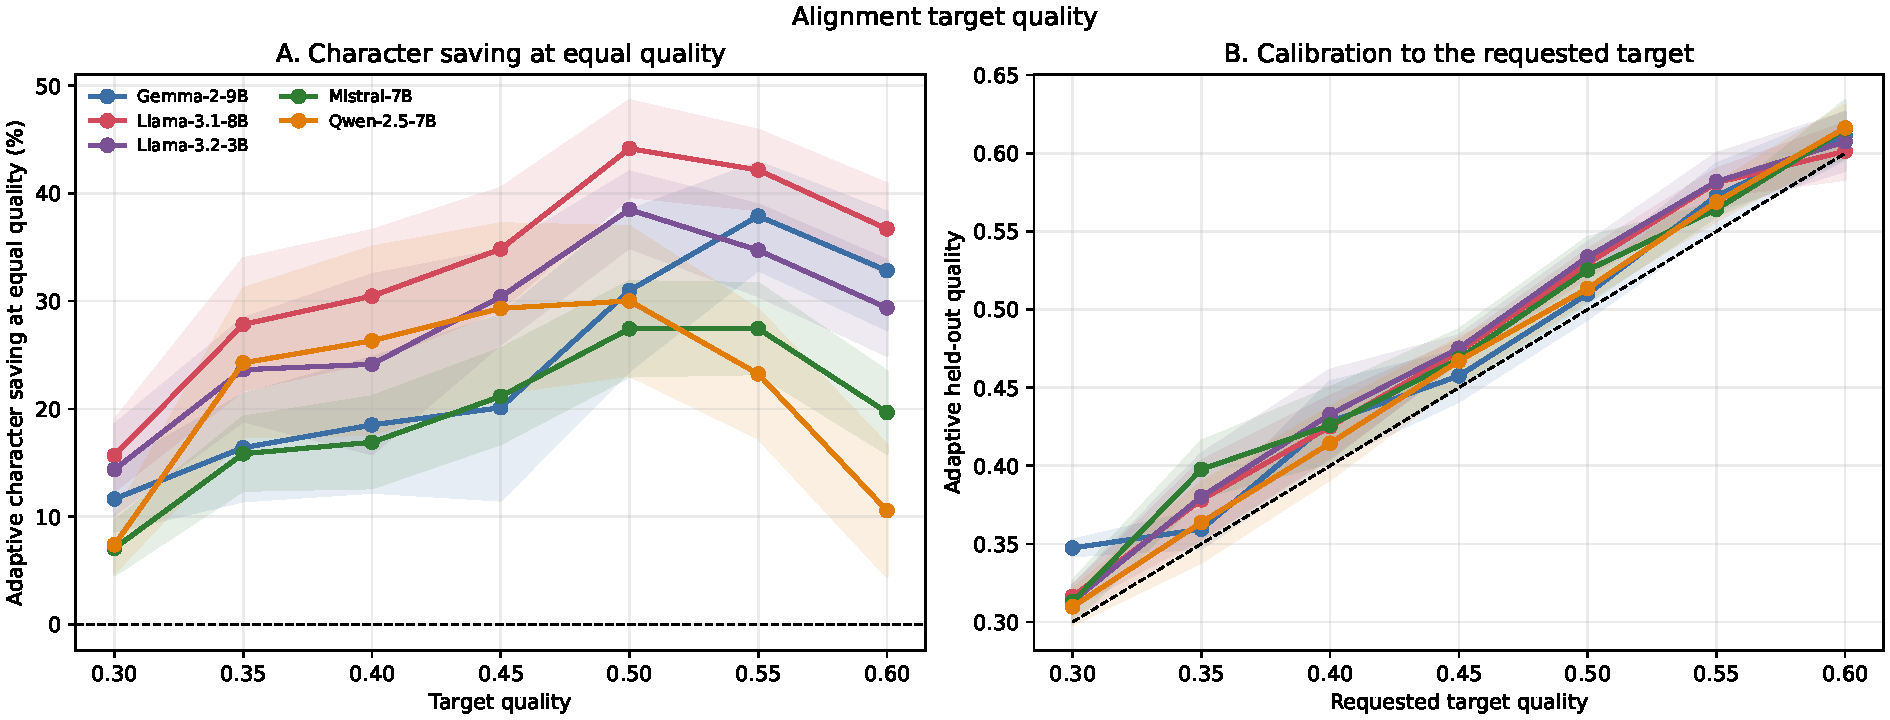
\includegraphics[width=\textwidth]
   {figures/alignment/alignment_target_quality_train_selected.pdf}
 \caption{Alignment target-quality results.  Left: adaptive character saving
 against the post-hoc minimum-cost non-adaptive Fixed-$N$ oracle subject to
 exactly the adaptive rule's expected held-out quality.  The oracle randomizes
 over at most two fixed counts before generation.  Right: adaptive held-out
 quality versus the requested target; the diagonal denotes exact calibration.
 Bands are 95\% intervals across ten splits.}
 \label{fig:alignment-target}
\end{figure}

The right panel shows the target-transfer error directly; the adaptive rule's
mean absolute held-out deviation from the requested target is 2.49 percentage
points.  The equal-quality diagnostic in the left panel removes that mismatch
from the cost comparison.  Averaged over
the five generators, adaptive character savings at targets 0.30 through 0.60
are respectively 11.22\%, 21.59\%, 23.26\%, 27.17\%, 34.22\%, 33.10\%, and
25.82\%.  All 35 generator--target cells are positive, with a 25.20\% mean
saving across cells.  The matched expected quality agrees with adaptive
quality to numerical precision in every one of the 350 split-level
comparisons.  These larger, uniformly positive values isolate adaptive
allocation efficiency, but they are oracle diagnostics because their two
Fixed-$N$ endpoints and mixing weight minimize character cost on the test
curve.


\section{Coding}
\label{sec:coding}

\subsection{Exact coding policy}
\label{sec:coding-algorithm}

The coding rule uses the same crossing logic, but it has a separate learning
procedure because correctness labels are available on the training problems.
That procedure returns a monotone score-to-correctness map and one global
shifted-exponential upper-tail model.  The stopping procedure freezes both
objects, maps each observed test score to calibrated probability, and finds a
fair cap under an optimistic version of the learned tail.  There is no online
local-tail fit and no divisor-specific configuration table.

\begin{algorithm}[H]
\caption{Coding: learn the calibrated law, then stop at its fair cap}
\label{alg:coding}
\footnotesize
\begin{algorithmic}[1]
\Procedure{LearnCodingLaw}{$\{(Y_{ij},Z_{ij}):i\in\mathcal A,j\le512\}$}
  \State Fit the monotone calibration map $\widehat g$ in
         Eq.~\eqref{eq:isotonic-map}
  \State Apply $\widehat g$ to the training scores to obtain calibrated
         correctness probabilities $P_{ij}=\widehat g(Y_{ij})$
  \State For each training problem, fit a shifted exponential to the
         inclusive upper quarter of its calibrated probabilities
  \State Average the fitted shifts and scales to obtain the global tail
         $\widehat F^{\rm tail}=\operatorname{ShiftedExp}(\bar\ell,\bar s)$
  \State \Return the frozen calibration $\widehat g$ and tail parameters
         $(\bar\ell,\bar s)$
\EndProcedure
\Statex
\Procedure{StopCoding}{$\widehat g,\bar\ell,\bar s,D_{\rm res}$}
  \Require Horizon $H=512$; initial count $m_0=3$; confidence
           $\gamma$ (default $0.8$); confidence level $\delta$ (default $0.05$)
  \State Generate $m_0$ programs, observe $(Y_j,K_j)$, and set
         $P_j\gets\widehat g(Y_j)$ for $j\le m_0$
  \State $n\gets m_0$
  \While{$n<H$}
    \State $v_n\gets\max_{j\le n}P_j$
           \Comment{best calibrated correctness probability}
    \State $m_n\gets\bigl|\{j\le n:P_j\ge
           Q_{0.75}(P_1,\ldots,P_n)\}\bigr|$
           \Comment{observed upper-tail count}
    \State $h_n\gets\sqrt{\log(1/\delta)/m_n}$
    \State $\ell_n^+\gets\operatorname{clip}_{[0,1]}
           (\bar\ell+\gamma\bar s h_n)$
           \Comment{optimistic tail shift}
    \State $s_n^+\gets\bar s(1+\gamma h_n)$
           \Comment{optimistic tail scale}
    \State $\rho_n\gets0.25(m_0/n)$ \Comment{regularized upper-tail mass}
    \State Define $\widehat F_n$: with probability $\rho_n$, draw
           $U\sim\operatorname{ShiftedExp}(\ell_n^+,s_n^+)$ conditioned on
           $U\le1$
    \Statex \hspace{\algorithmicindent}Otherwise set $U=0$
    \State $c_n\gets(nD_{\rm res})^{-1}\sum_{j=1}^{n}K_j$
           \Comment{estimated cost of one more program}
    \State $\displaystyle \tau_n\gets\inf\left\{t\in[0,1]:
           \mathbb E_{U\sim\widehat F_n}[(U-t)_+]\le c_n\right\}$
           \Comment{fair cap of the calibrated law}
    \If{$v_n\ge\tau_n$}
      \State \textbf{break} \Comment{incumbent has reached the fair cap}
    \EndIf
    \State Generate program $n+1$, observe $(Y_{n+1},K_{n+1})$, and set
           $P_{n+1}\gets\widehat g(Y_{n+1})$
    \State $n\gets n+1$
  \EndWhile
  \State $J\gets\min\arg\max_{j\le n}P_j$
  \State \Return program $J$ and the exact opened character count
         $\sum_{j=1}^{n}K_j$
\EndProcedure
\end{algorithmic}
\end{algorithm}

\paragraph{Computing the coding fair cap.}
The upper-quarter exponential fit in the learning procedure is exact shorthand
for $\ell_i=Q_{0.75}(P_{i1},\ldots,P_{iH})$ and
$s_i=\max\{\operatorname{mean}_{j:P_{ij}\ge\ell_i}
(P_{ij}-\ell_i),10^{-8}\}$, followed by
$\bar\ell=\operatorname{mean}_i\ell_i$ and
$\bar s=\operatorname{mean}_i s_i$.  The mass
$\rho_n=0.25(3/n)$ incorporates both the fitted upper-quarter mass and the
implementation's smooth opportunity-decay factor.  Consequently the fair-cap
test is algebraically identical to the former expected-gain calculation; the
32-point quadrature is only how the implementation evaluates the expectation,
not an additional algorithmic decision.

For utility, one development-selected multiplier sets
$D_{\rm res}=0.85D$ at every economic divisor $D$.  This changes only the
reservation comparison; evaluation always records binary correctness minus
the exact opened character count divided by $D$.  For target accuracy,
$D_{\rm res}$ is the frozen target-specific divisor described below and the
reported outcome is correctness together with exact characters.  Thus the old
ten-row divisor-specific configuration table is replaced by the two procedures
in Algorithm~\ref{alg:coding}.  The only terminal cap is the absolute
512-program data boundary.

\subsection{Utility experiment and fixed-policy baselines}
\label{sec:coding-experiment}

We evaluate ten final 41/42 splits, with 48 random permutations for every
test problem.  Each candidate pool contains 512 programs.  For each split,
the isotonic map and global tail use only the 41 training
problems.  The adaptive configuration and $D_{\rm res}$ for every economic
divisor were frozen before final split IDs 75--84.  Development split IDs
63--67 selected the single multiplier $D_{\rm res}/D=0.85$; no final split
selected a tail model or divisor-specific parameter.  The final evaluation
uses binary correctness minus exact cumulative characters divided by $D$.

We compare against three baselines.

\paragraph{1. Train-selected Fixed-$N$ (implementable).}
For each outer split and divisor, choose the integer $N$ that maximizes mean
correctness minus character cost on the 41 training problems.  Freeze $N$ and
evaluate it on the 42 test problems with the same permutations used for the
adaptive policy.

\paragraph{2. Test-oracle Fixed-$N$.}
Choose the integer $N\in\{1,\ldots,512\}$ that maximizes the same utility on
the current test problems and permutations.  This is a post-hoc upper
envelope for uniform Fixed-$N$, not a deployable method.

\paragraph{3. Train-selected fixed character budget (implementable).}
For each split and divisor, use 48 deterministic permutations of the 41
training problems to select one global threshold $R$.  The policy opens one
program and continues while the cumulative characters already observed are
at most $R$.  We choose $R$ to maximize training mean correctness minus exact
character cost, enumerating every observed training-prefix breakpoint so the
optimization is exact.  We then freeze $R$ and apply the same stopping rule
to the 42 test problems.  The rule neither predicts the next program length
nor reads test outcomes; because the final program is charged in full, its
realized total may exceed $R$ by that program's length.

Figure~\ref{fig:coding-baselines} and Table~\ref{tab:coding-results} use the
percentage relative improvement in Eq.~\eqref{eq:relative-improvement}.
The mean splitwise improvement over the train-selected baseline is positive
at every displayed divisor and averages 2.63\%.  Against test-oracle Fixed-$N$, it averages
$-0.12\%$: the mean is positive at five divisors and negative at five.  This is the more
demanding comparison because the oracle selects $N$ after seeing evaluation
outcomes, whereas adaptive stopping changes its stopping time problem by
problem using only the observed prefix.  Relative to the train-selected fixed
character budget, adaptive utility improves by 3.48\% on average.  Its
mean improvement is positive at all ten divisors, and six of the ten 95\%
intervals lie entirely above zero.

\begin{figure}[H]
 \centering
 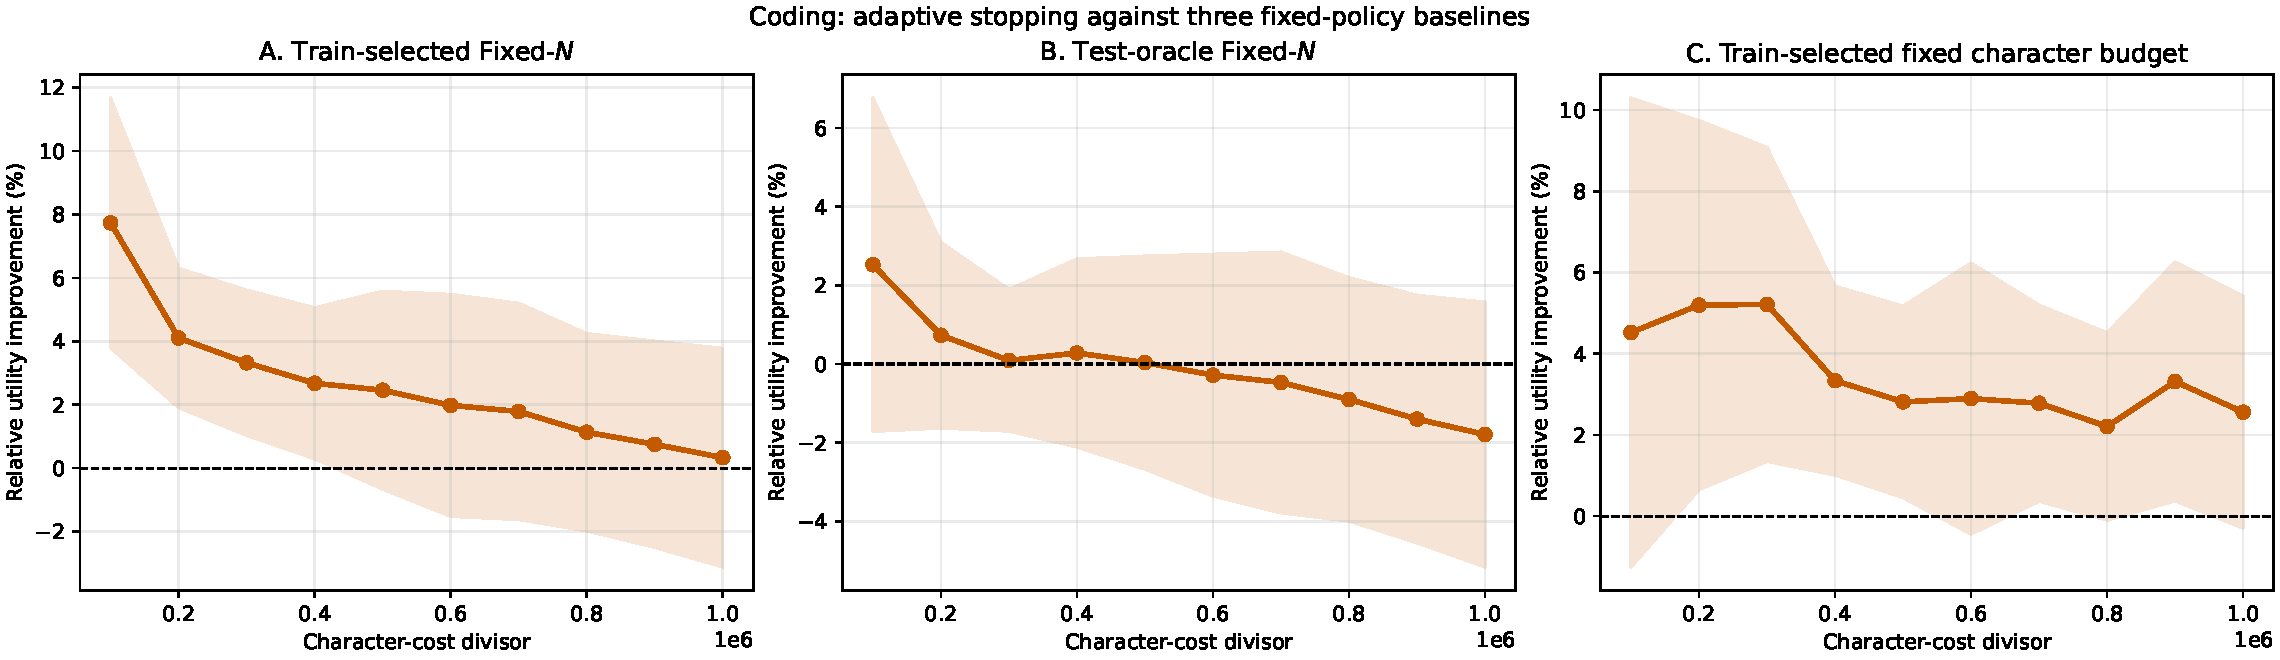
\includegraphics[width=\textwidth]
   {figures/coding/coding_revised_baselines.pdf}
 \caption{Coding percentage relative utility improvement over train-selected
 Fixed-$N$, test-oracle Fixed-$N$, and the train-selected fixed character
 budget.  Bands are pointwise 95\% Student-$t$ intervals over ten final
 problem splits; the dashed zero line denotes equal utility.}
 \label{fig:coding-baselines}
\end{figure}

\begin{table}[H]
\centering
\small
\begin{tabular}{rccc}
\toprule
Character divisor $D$ & Train-selected $N$ & Test-oracle $N$ & Fixed char. budget\\
\midrule
100,000   & $+7.73\%$ & $+2.52\%$ & $+4.52\%$\\
200,000   & $+4.10\%$ & $+0.73\%$ & $+5.20\%$\\
300,000   & $+3.32\%$ & $+0.09\%$ & $+5.21\%$\\
400,000   & $+2.68\%$ & $+0.28\%$ & $+3.34\%$\\
500,000   & $+2.46\%$ & $+0.04\%$ & $+2.81\%$\\
600,000   & $+1.98\%$ & $-0.28\%$ & $+2.89\%$\\
700,000   & $+1.79\%$ & $-0.47\%$ & $+2.78\%$\\
800,000   & $+1.13\%$ & $-0.90\%$ & $+2.21\%$\\
900,000   & $+0.75\%$ & $-1.40\%$ & $+3.31\%$\\
1,000,000 & $+0.33\%$ & $-1.79\%$ & $+2.56\%$\\
\midrule
Mean & $+2.63\%$ & $-0.12\%$ & $+3.48\%$\\
\bottomrule
\end{tabular}
\caption{Coding percentage relative utility improvement over ten final
splits.  The fixed character budget is selected only on the training half
and then frozen for test.}
\label{tab:coding-results}
\end{table}


\subsection{Target accuracy and character saving}
\label{sec:coding-target}

For each 41/42 split and requested accuracy in $\{0.25,0.30,0.35\}$, the
isotonic map is fit on the 41 training problems.  The Fixed-$N$ baseline is
the minimum-character integer $N$ that reaches the requested accuracy on that
same training half; that $N$ is then frozen for test.  The adaptive target
selector uses exactly Algorithm~\ref{alg:coding} but replaces $0.85D$ by one
reservation divisor chosen from
$\{25{,}000,35{,}000,\ldots,10{,}000{,}000\}$.  Development split IDs 55--59
freeze the mean held-out accuracy and geometric-mean character cost at each
divisor.  For a requested accuracy, the selector takes the cheapest divisor
whose development accuracy reaches the target: 25,000, 140,000, and
2,800,000 for the three reported targets.  There is no current-split blend,
configuration search, safety margin, interpolation, or policy mixture in the
adaptive rule.  The outer 41-problem training half is still the only source
for its isotonic map and global tail.

\begin{figure}[H]
 \centering
 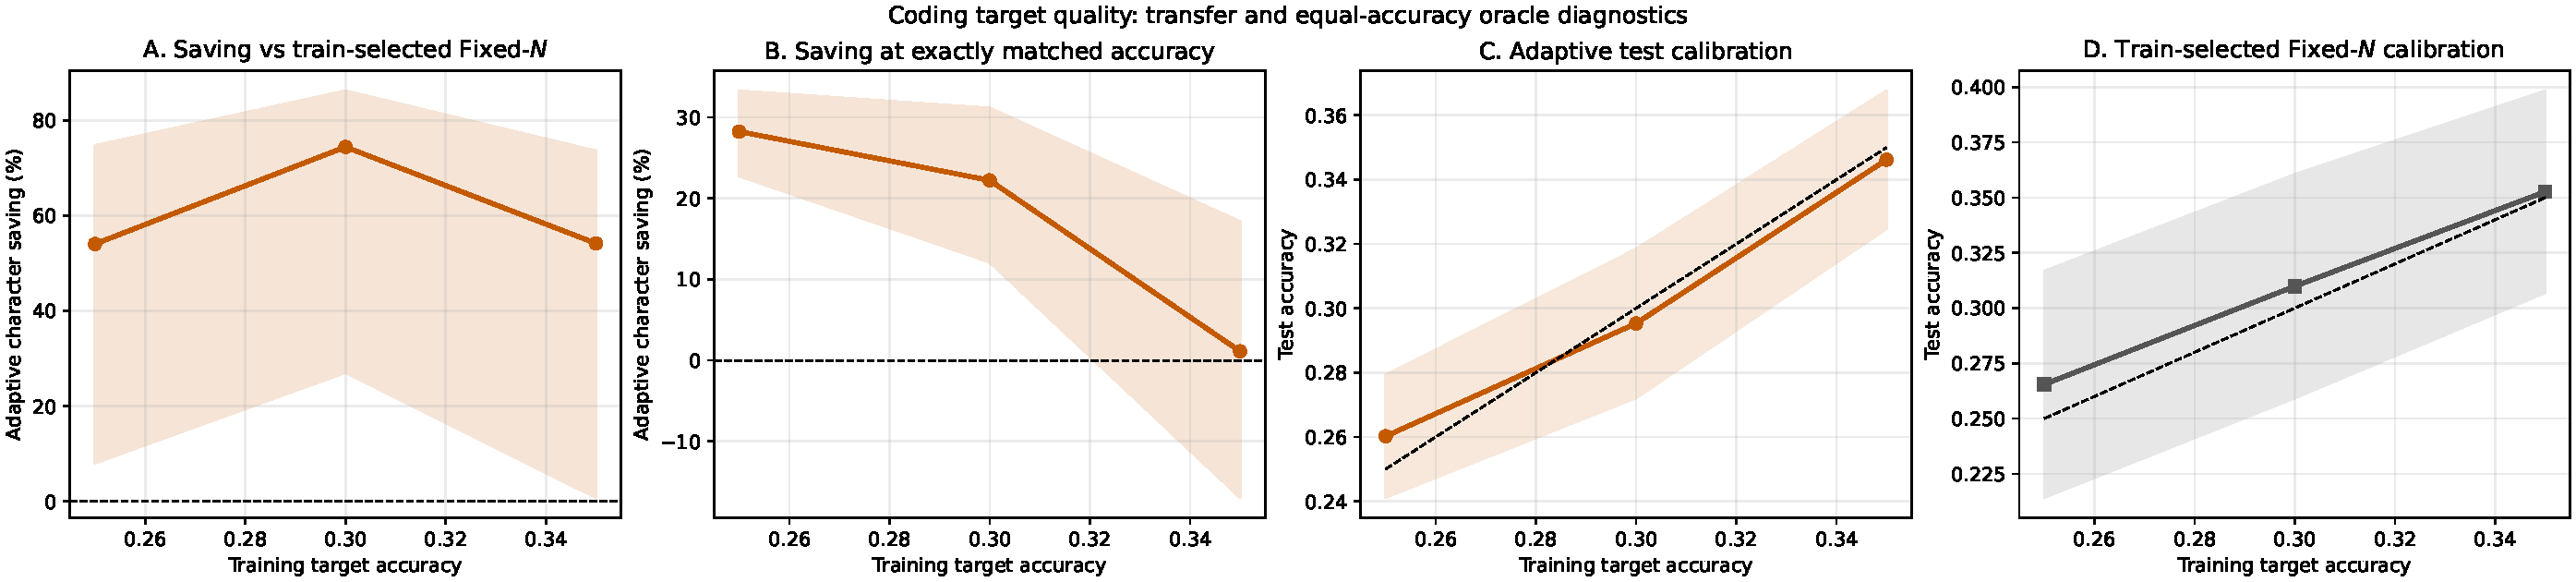
\includegraphics[width=\textwidth]
   {figures/coding/coding_target_quality_train_selected.pdf}
 \caption{Coding target-accuracy results.  A: aggregate adaptive character
 saving relative to train-selected Fixed-$N$.  B: saving relative to the
 post-hoc non-adaptive Fixed-$N$ randomization with exactly the adaptive
 aggregate test accuracy.  C--D: held-out calibration of the adaptive and
 train-selected Fixed-$N$ rules.  The diagonal is exact target transfer; bands
 are 95\% intervals across ten splits.}
 \label{fig:coding-target}
\end{figure}

At targets 0.25, 0.30, and 0.35, adaptive test accuracies are 0.260, 0.295,
and 0.346, while train-selected Fixed-$N$ obtains 0.265, 0.310, and 0.353.
Aggregate character savings are 54.04\% (95\% interval 8.06--74.71\%),
74.41\% (27.04--86.19\%), and 54.17\% (0.83--73.58\%).  Thus the simplest
selector overshoots the first target by 1.02 points and undershoots the latter
two by 0.47 and 0.38 points.  The calibration panels remain essential: cost
savings are results for policies selected before test, not a claim that their
realized test accuracies are identical.

For the equal-accuracy diagnostic, we first average the exact held-out
Fixed-$N$ accuracy and character curves over the ten final splits.  We then
choose the minimum-character non-adaptive rule whose average accuracy equals
the adaptive average.  Because an integer $N$ will almost never hit a decimal
accuracy exactly, this rule randomizes between two adjacent counts before any
program is generated.  The selected pairs and high-count probabilities are
$(8,9;0.158)$, $(18,19;0.603)$, and $(77,78;0.451)$ for the three targets.
Their aggregate accuracies are 0.260218, 0.295288, and 0.346181, equal to the
adaptive accuracies to numerical precision.

Adaptive/fixed expected character counts at those matches are
2,967/4,136, 7,334/9,431, and 38,823/39,265.  Thus adaptive character savings
are 28.26\%
(95\% interval 22.77--33.29\%), 22.24\% (12.15--31.17\%), and 1.13\%
($-16.92$--17.15\%).  Thus coding has a clear equal-accuracy cost advantage at
the first two targets, while the data do not establish an advantage at 0.35.
This diagnostic is deliberately non-implementable because its counts and
mixing weights are selected from the final test curves.  It affects only the
comparator; Algorithm~\ref{alg:coding} remains one deterministic adaptive
stopping rule.

\subsection{Evaluation boundary}

Alignment uses cached responses from 100 prompts per generator.  Coding is
conditioned on being solved by at least one of 512 cached programs, so it does
not describe the excluded all-incorrect problems.  Its development,
validation, and final splits resample the same 83 problems rather than
disjoint corpora.  Coding utility uses final split IDs 75--84, and coding
target quality uses IDs 95--104; selectors do not read their current final
split.  This is within-corpus repeated-split evidence, not evaluation on new
identities.  The utility multiplier and target profile are frozen on separate
development splits; every test oracle is post-hoc.


\section{Discussion}

The theoretical and practical rules share one idea: continue while the value
of another reward draw above the incumbent exceeds mean opening cost.  The
LLM implementations estimate both sides on a common scale.  Alignment uses
relative BT utility and a current-prompt tail, so its adaptive rule requires
no training data.  Coding uses a train-only isotonic correctness probability
and one global upper-quarter tail.  Response length represents unknown cost,
is predicted by the observed-prefix mean without looking ahead, and is
charged exactly after generation.

Train-selected Fixed-$N$ is deployable; test-oracle Fixed-$N$ removes transfer
error in choosing one common count.  The alignment character-budget oracle is
stronger still: it knows prompt-specific mean lengths and allocates different
counts.  Adaptive stopping beats both Fixed-$N$ baselines on average, whereas
the cost-aware oracle exposes room to improve length prediction.  Equal-cost
alignment results separately show a quality advantage at fixed expected
characters.  In coding, adaptive stopping also outperforms the character-only
budget selected on the training half.

Target attainment is harder: the divisor or integer $N$ is selected before
test, then quality moves with the held-out problems.  Fixed-$N$ transfers more
accurately than the current alignment divisor grid.  In coding, the frozen
development inverse curve is close at all three targets but modestly
overshoots the first and undershoots the other two.  Cost savings therefore
require calibration panels---without matched test quality they are not, by
themselves, an efficiency comparison.  The post-hoc equal-quality diagnostics
remove that ambiguity.  Alignment retains positive savings in every
generator--target cell.  Coding retains clear savings at targets 0.25 and
0.30, but its apparent advantage at 0.35 shrinks to 1.13\% with an interval
spanning zero.

The theorem does not certify these exponential tail fits; that would require
finite-sample fair-cap concentration under reward-model error and length
variation.  The experiments instead test the fitted crossing rule end to end,
providing empirical support and motivating a sharper joint analysis.  The
simplification study is nevertheless informative: eliminating the alignment
prior and collapsing coding's divisor-specific grid to one formula changes
mean utility by only $-0.00040$ and $-0.00057$, respectively, on the held-out
confirmations.


\end{document}
